%
% File acl2012.tex
%
% Contact: Maggie Li (cswjli@comp.polyu.edu.hk), Michael White (mwhite@ling.osu.edu)
%%
%% Based on the style files for ACL2008 by Joakim Nivre and Noah Smith
%% and that of ACL2010 by Jing-Shin Chang and Philipp Koehn


\documentclass[11pt,letterpaper]{article}
\usepackage[letterpaper]{geometry}
\usepackage{acl2012}
\usepackage{times}
\usepackage{latexsym}
\usepackage{graphicx}
\usepackage{amssymb}
\usepackage{amsmath}
\usepackage{multirow}
\usepackage{url}
\usepackage{tipa}
\makeatletter
\newcommand{\@BIBLABEL}{\@emptybiblabel}
\newcommand{\@emptybiblabel}[1]{}
\makeatother
\usepackage[hidelinks]{hyperref}
\DeclareMathOperator*{\argmax}{arg\,max}
\setlength\titlebox{6.5cm}    % Expanding the titlebox

\title{Discovering Cognates Using LSTM Networks}

\author{First Author \\
  Affiliation / Address line 1 \\
   Affiliation / Address line 2 \\
   Affiliation / Address line 3 \\
   {\tt email@domain} \\\And
   Second Author \\
   Affiliation / Address line 1 \\
   Affiliation / Address line 2 \\
   Affiliation / Address line 3 \\
   {\tt email@domain} \\}

%\author{Shantanu Kumar \and Ashwini Vaidya \and Sumeet Agarwal \\ 
%  Indian Institute of Technology Delhi
%  \\ {\tt \{ee1130798, ird11278, sumeet\}@iitd.ac.in}}

\date{}

\begin{document}
\maketitle

%%%%%%%%%%%%%%%%%%%%%%%%%%%%%%%%%%%%%%%%%%%%%%%%
\begin{abstract}
In this paper, we present a deep learning (DL) model for the task of pairwise cognate prediction, i.e. identifying whether English `\textit{Night}' and German `\textit{Nacht}', both meaning \textit{Night} come from the same common ancestor. We use a character level model with recurrent neural network architecture and attention and test its performance on datasets drawn from three different language families. Our results show an improvement in performance as compared to existing models and highlight the usefulness of phonetic and conceptual features. We also employ our model to the domain of discovering similar word pairs from a pair of closely related languages to bootstrap lexical resource creation.
\end{abstract}

%%%%%%%%%%%%%%%%%%%%%%%%%%%%%%%%%%%%%%%%%%%%%%%%
\section{Introduction}
Cognates are words across different languages that are known to have originated from the same word in a common ancestral language. For example, the English word  `\textit{Night}' and the German word `\textit{Nacht}', both meaning \textit{Night} and English `\textit{Hound}' and German `\textit{Hund}', meaning \textit{Dog} are cognates whose origin can be traced back to Proto-Germanic. Cognate words are not simply the translations of each other in any two languages, but are historically known to have a common origin. For example, the English word `\textit{Hound}' and the Spanish word `\textit{Perro}' both mean \textit{Dog} but are not cognates.

Traditionally, the identification of cognates was carried out by historical linguists, using word lists and establishing sound correspondences between words. These are useful in determining linguistic distance within a language family, and also to understand the process of language change. Cognate information has also been used in several downstream NLP tasks, like sentence alignment in bi-texts \cite{simard1993using} and improving statistical machine translation models \cite{kondrak2003cognates}. Additionally, it has been proposed that cognates can be used to share lexical resources among languages that are closely related \cite{Singh:07b}.

For some time now, there has been a growing interest in automatic cognate identification techniques. Most approaches for this task focus on finding similarity measures between a pair of words such as orthographic or phonetic similarity \cite{hauer2011clustering,inkpen2005similarity,List2016g}. These are used as features for a classifier to identify cognacy between a given word-pair.  
For instance, Rama~\shortcite{rama2015automatic} attempt to identify cognates by looking at the common subsequences present in the candidate word pair.

For a cognate pair like the English `\textit{Wheel}' and the Sanskrit `\textit{Chakra}', such an approach fails as they have nothing in common with each other orthographically. In fact, even for a pair like English `\textit{Father}' and Latin `\textit{Pater}', a common subsequence approach completely ignores the similarity between the `\textit{Fa}' and `\textit{Pa}' phonemes, which is a possible indication of cognacy between the pair. Such surface similarity measures miss out on capturing generalizations beyond string similarity, as cognate words are not always revealingly similar. 

Thus, there is a need for information about phonological similarity that is beyond surface similarity, such as the sound correspondences that are used in historical linguistics to narrow down candidate pairs as cognates.

%%%%%%%%%%%%%%%%%%%%%%%%%%%
\begin{table*}[ht]
\centering
\begin{tabular}{llcccccc}
\multicolumn{1}{c}{\textbf{}}                           & \multicolumn{1}{c}{\textbf{}}         & \multicolumn{6}{c}{\textbf{Concept}}                                                                      \\ \cline{3-8} 
\multicolumn{1}{c}{}                                    & \multicolumn{1}{c}{\textit{}}         & \multicolumn{2}{c}{\textit{ALL}} & \multicolumn{2}{c}{\textit{BIG}} & \multicolumn{2}{c}{\textit{ANIMAL}} \\ \cline{3-8} 
\multicolumn{1}{l|}{\multirow{4}{*}{\textbf{Language}}} & \multicolumn{1}{l|}{\textit{ENGLISH}} & all   & \multicolumn{1}{c|}{001} & big   & \multicolumn{1}{c|}{009} & animal   & \multicolumn{1}{c|}{015} \\ \cline{3-8} 
\multicolumn{1}{l|}{}                                   & \multicolumn{1}{l|}{\textit{FRENCH}}  & tut   & \multicolumn{1}{c|}{002} & grand & \multicolumn{1}{c|}{010} & animal   & \multicolumn{1}{c|}{015} \\ \cline{3-8} 
\multicolumn{1}{l|}{}                                   & \multicolumn{1}{l|}{\textit{MARATHI}} & serve & \multicolumn{1}{c|}{006} & motha & \multicolumn{1}{c|}{011} & jenaver  & \multicolumn{1}{c|}{017} \\ \cline{3-8} 
\multicolumn{1}{l|}{}                                   & \multicolumn{1}{l|}{\textit{HINDI}}   & seb   & \multicolumn{1}{c|}{006} & bara  & \multicolumn{1}{c|}{012} & janver   & \multicolumn{1}{c|}{017} \\ \cline{3-8} 
\end{tabular}
\label{sample_wordlist}
\caption{Sample Word List from the Indo-European Dataset}
\end{table*}

%%%%%%%%%%%%%%%%%%%%%%%%%%%


By using DL based models, the need for external feature engineering is circumvented as the system learns to find hidden representations of the input depending on the task in hand. We make use of an end-to-end character-level recurrent neural network (RNN) based model that is adapted from a model used on a word-level entailment task \cite{rocktaschel2016reasoning}. Our model is able to outperform both the common subsequence model \cite{rama2015automatic} as well as a recent CNN-based model \cite{rama2016siamese} on the task. 

LSTM (Long Short Term Memory) networks are being used in an extensive range of NLP tasks to build end-to-end systems. LSTMs have been successfully applied to machine translation \cite{bahdanau2014neural}, language modelling \cite{mikolov2010recurrent}, information retrieval \cite{sordoni2015hierarchical} and RTE \cite{snli:emnlp2015}. In the subsequent sections, we describe our LSTM based Siamese-style architecture which uses character by character attention to enrich the representations of the input word pairs. We compare our model against existing supervised approaches. We also demonstrate the importance of the attention layer and the role of word semantics in the task, and examine how the properties of the datasets specifically with respect to size and transcription affect the models.

The task of discovering cognates can be particularly useful among the languages of South Asia, which are not rich in lexical resources. Information about cognates can become an important source for assisting the creation and sharing of lexical resources between languages. Therefore, another contribution of this work is to apply our cognate detection model to a real language pair. We apply our model to the domain of Hindi-Marathi, using a large unlabelled corpus of aligned texts to find cognate pairs.

%%%%%%%%%%%%%%%%%%%%%%%%%%%%%%%%%%%%%%%%%%%%%%%%
\section{Problem Statement}

The task of cognate identification will make use of word lists from different language families taken from the basic vocabulary e.g.  kinship terms, body parts, numbers etc. Usually this vocabulary will represent concepts from the language itself and not borrowed items, (although this is also possible at times). Table~\ref{sample_wordlist} shows a part of a word list that is used for the task. Each cell in the table contains a lexical item belonging to a particular language and a particular concept, along with its cognate class ID. If two words have the same cognate class ID, then they are identified as cognates.

The task of pairwise cognate prediction can thus be more formally defined as follows:  given two words from a word list, belonging to different languages but to the same concept, predict whether the words in the pair are cognates. Thus, a model for this task would take as input a candidate pair of words and produce as output a single value classifying the pair as cognate or non-cognate. 

%%%%%%%%%%%%%%%%%%%%%%%%%%%%%%%%%%%%%%%%%%%%%%%%
\section{Model}

\begin{figure}[t]
	\centering
	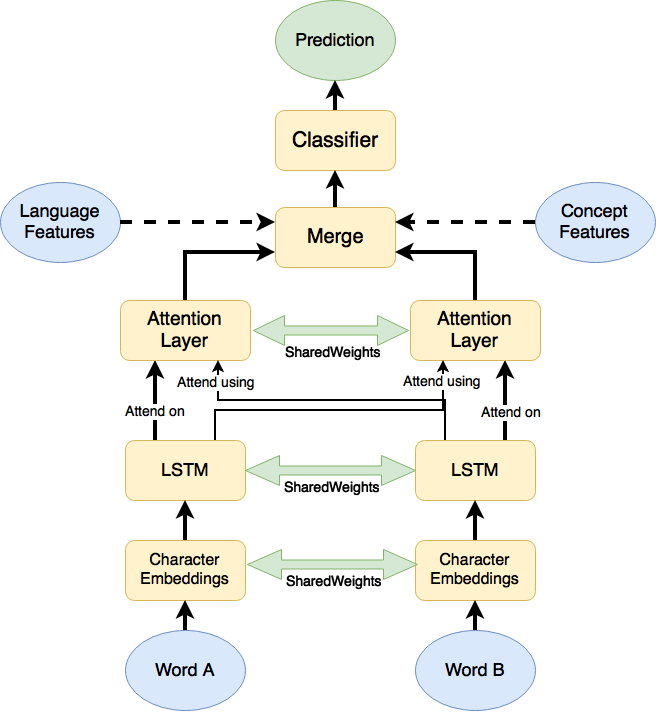
\includegraphics[width=0.45\textwidth]{CoAttNetwork}
    \caption{Recurrent Co-Attention Network for Cognate Discovery}
    \label{CoAttNet}
\end{figure}

The overall model used in our system is called the Recurrent Co-Attention Model (\textit{CoAtt}). It is adapted from the word-by-word attention model used by \cite{rocktaschel2016reasoning} for the task of recognising textual entailment (RTE) in natural language sentences. Just as the RTE task involves understanding the semantics of a sentence which is hidden behind sequence of words, the cognate identification task also requires information beyond surface character similarity, which was the motivation to adapt this particular model for our task. The network is illustrated in Figure~\ref{CoAttNet}. We have converted the RTE model into a siamese-style network that encodes a word pair in parallel and then makes a discriminative judgement in the final layer. 

The input words are first encoded into character level embeddings followed by a bidirectional LSTM network and finally a character by character attention layer as described the subsections that follow. The encodings of both the words are merged and passed through a 2-layer neural network classifier with \textit{tanh} and \textit{sigmoid} activations to make a final binary prediction. Additionally, we also add a \textit{Language features} vector or a \textit{Concept features} vector to the model by concatenating it with the merged attention vector before passing it to the 2-layer neural network.

%%%%%%%%%%%%%%%%%%%%%%
\subsection{Character Embeddings}

The input words are first encoded into character level embeddings. Character embeddings are a form of distributional representation, where every character of the vocabulary is expressed as a vector in a vector space. This is done using a character level embedding matrix $E \in \mathbb{R}^{n_e \times |C|}$. Here $n_e$ is the dimensionality of the embeddings and $C$ is the vocabulary of all characters. Thus for an input word $x$ which can be represented as sequence of characters $x = \{c_{i_1}, c_{i_2}, ..., c_{i_n}\}$, is transformed into a sequence of vectors $y = \{e_{i_1}, e_{i_2}, ..., e_{i_n}\}$ where $e_j$ is the $j^{th}$ column of the $E$ matrix. This embedding matrix is learnt during training and each column in the matrix represents the embedding vector of the respective token in the vocabulary. 

There are two ways of initialising the character embedding matrix for training. The matrix can be \textit{randomly initialised} by sampling values from a uniform distribution. In such a case, the embeddings are dependent heavily on the training and the random vectors assigned to each character can change during training to such values that are optimal for the task. The other method of initialising the embeddings matrix is by using \textit{phonetic feature vectors} (PV). These phonetic vectors are manually defined binary vectors that are based on various linguistic properties of phonemes such as place of articulation (Dental, Nasal) and manner of articulation (Fricative, Voiced, Lateral). We adapted these feature vectors from Rama~\shortcite{rama2016siamese} after some minor corrections.

%%%%%%%%%%%%%%%%%%%%%%
\subsection{LSTM}

After the input words to the network are transformed using the character embedding matrix, we encode them with an LSTM. Given an input word $y = \{e_1, e_2, ..., e_n\}$, at every time step $t$ the LSTM of hidden unit size $n_h$ uses the next input $e_t$, the previous output $h_{t-1}$ and the previous cell state $c_{t-1}$ to compute the next output $h_t$ and the next cell state $c_t$ as follows,

\begin{align}
H &= [e_t \enspace h_{t-1}] \\
i_t &= \sigma (W^iH + b^i) \\
o_t &= \sigma (W^oH + b^o) \\
f_t &= \sigma (W^fH + b^f) \\
c_t &= i_t * tanh(W^cH + b^c) + f_t * c_{t-1} \\
h_t &= o_t * tanh(c_t)
\end{align}

Here $W^i$, $W^o$, $W^f$, $W^c \in  \mathbb{R}^{n_e+n_h \times n_h}$ and $b_i$, $b_o$, $b_f$, $b_c \in \mathbb{R}^{n_h}$ are trained weights of the LSTM. $[\enspace]$ is the concatenation operator and $\sigma$ is the element-wise sigmoid opertor. The final output of the LSTM gives us a sequence $\{h_1, h_2, ..., h_n\}$ for each word, where $h_j \in \mathbb{R}^{n_h}$.

%%%%%%%%%%%%%%%%%%%%%%
\subsection{Attention Layer}

Attention neural networks have been used extensively in tasks like machine translation \cite{mtattention}, image captioning \cite{cpattention} and visual question answering \cite{stackedattention}. At a high level, attention can be considered as a soft selection procedure, where given a sequence of inputs, one would like to focus or attend on the important part of the sequence with respect to a context. We use this procedure to enhance the representation of the character sequence of a word coming out of the LSTM, by giving it as context the second word. One can compare the attention mechanism with the common subsequence model. In a common subsequence model, one makes a hard selection procedure by using as features only the common subsequences of both the words. In the attention model, the network makes a soft selection while focusing on those parts of the sequence which are important with respect to the other word.

Given a character vector $h \in  \mathbb{R}^{n_h}$ using which we would like to attend on a sequence of character vectors $Y = \{c_1, c_2, ..., c_L\} \in \mathbb{R}^{n_h \times L}$, we generate a set of attention weights $\alpha$ and an attention-weighted representation $r \in  \mathbb{R}^{n_h}$ of $Y$ as,

\begin{align}
M &= tanh(W^yY + W^hh\otimes e_L) \\
\alpha &= softmax(w^TM) \\
r &= Y\alpha_t^T
\end{align}

The outer product $W^hh\otimes e_L$ repeats the linearly transformed $h$ as many times as there are characters in $Y$ ($L$ times). Using the mechanism followed by Rockt\"aschel et al.~\shortcite{rocktaschel2016reasoning} for word-by-word attention, we employ a character-by-character attention model, wherein we find an attention weighted representation of the first word $Y = \{c_1, c_2, ..., c_L\} \in \mathbb{R}^{n_h \times L}$ at every character of the second word $H = \{h_1, h_2, ..., h_N\} \in \mathbb{R}^{n_h \times N}$.

\begin{align}
M_t &= tanh(W^yY + (W^hh_t + W^rr_{t-1})\otimes e_L) \\
\alpha_t &= softmax(w^TM_t) \\
r_t &= Y\alpha_t^T + tanh(W^tr_{t-1})
\end{align}

Here $W^y$, $W^h$, $W^r$, $W^t \in  \mathbb{R}^{n_h \times n_h}$ and $w \in \mathbb{R}^{n_h}$ are trained weights of the Attention layer. The final output gives us $r_N = r_{YH}$ which is the attention weighted representation of $Y$ with respect to $H$. Similarly, we also obtain $r_{HY}$. The final feature vector $r^*$ that is passed to the multi-layer perceptron for classification is the concatenation of $r_{HY}$ and $r_{YH}$ vectors. This method of making both the character sequences attend over each is called the Co-Attention mechanism.
 
%%%%%%%%%%%%%%%%%%%%%%
\subsection{Language \& Concept Features}

It is known that some languages are more closely related to each other as compared to others. For example from Table~\ref{sample_wordlist} one can see that \textit{Hindi} is more related to \textit{Marathi} than to \textit{French}. That is a candidate word pair with words from \textit{Hindi} and \textit{Marathi} is more likely to be a cognate pair as compared to a word pair with words from \textit{Hindi} and \textit{French}. This information about language relatedness can be exploited by using as features a 2-hot encoding vector that represents the respective languages of the two input words. During training, the network can use these features to learn automatically which language pairs are closely related from the data.

Similar to language information, we hypothesise that information about the semantics of the input words can also be useful features for the classifier. The word semantics inherently contain information like the part-of-speech (POS) category of the word. Our initial exploration of the data showed that certain POS categories such as question words or prepositions tend to have greater divergence in their cognate classes as compared to nouns or adjectives. We use the GloVe word embedding \cite{pennington2014glove} for the English concept of the input word pair as the concept feature vector. Word embeddings are distributional representations of words in a low-dimensional space compared to the vocabulary size and they have been shown to capture semantic information about the words inherently. 

%%%%%%%%%%%%%%%%%%%%%%%%
\begin{table*}[ht]
\centering
\begin{tabular}{|l|c|c|c|c|}
\hline
\textbf{Language Family} & \textbf{Languages} & \textbf{Concepts} & \textbf{Unique Lexical Items} & \textbf{Cognate Classes} \\ \hline
Indo-European   & 52        & 208      & 8622                & 2528            \\
Austronesian    & 100       & 210      & 10079                & 4863            \\
Mayan           & 30        & 100      & 1629                 & 858          \\ \hline  
\end{tabular}
\caption{Statistics about the different language families}
\label{datastat}
\end{table*}

\begin{table*}[t]
\centering
\begin{tabular}{|l|cc|cc|cc|}
\cline{2-7}
\multicolumn{1}{c}{\textbf{}} & \multicolumn{2}{|c|}{\textbf{Indo-European}} & \multicolumn{2}{c|}{\textbf{Austronesian}} & \multicolumn{2}{c|}{\textbf{Mayan}} \\ \cline{2-7}
\multicolumn{1}{c|}{}          & \textit{Total}               & \textit{Positive}             & \textit{Total}               & \textit{Positive}            & \textit{Total}           & \textit{Positive}         \\ \hline
\textbf{Cross Language Evaluation}                      &                      &                      &                 &                &             &             \\
Training Samples              & 218,429             & 56,678               & 333,626             & 96,356              & 25,473          & 9,614            \\
Testing Samples               & 9,894               & 2,188                & 20,799              & 5,296               & 1,458           & 441             \\
                                                       &                      &                      &                 &                &             &             \\ \hline
\textbf{Cross Concept Evaluation}                      &                      &                      &                 &                &             &             \\
Training Samples              & 223,666             & 61,856               & 375,693             & 126,081             & 28,222          & 10.482           \\
Testing Samples               & 103,092             & 21,547               & 150,248             & 41,595              & 12,344          & 4,297                       \\ 
                                                       &                      &                      &                 &                &             &             \\ \hline
\end{tabular}
\caption{Number of word pairs obtained for both modes of evaluation from different language families}
\label{C_count}
\end{table*}

%%%%%%%%%%%%%%%%%%%%%%%%
%%%%%%%%%%%%%%%%%%%%%%%%%%%%%%%%%%%%%%%%%%%%%%%%
\section{Experiments}

In the subsections below we describe the datasets that we used and the comparisons we made with our models. This is followed by the three experiments we conducted with the datasets.

%%%%%%%%%%%%%%%%%%%%%%%%
\subsection{Datasets}

We make use of three datasets in our work which come from three language families. These families make a good test set as they vary widely in terms of the number of languages, concepts and cognate classes. The first and primary dataset that we use is the IELex Database, which contains cognacy judgements from the Indo-European language family. The dataset is curated by Michael Dunn\footnote{http://ielex.mpi.nl/}. Second, we include a dataset taken from the Austronesian Basic Vocabulary project \cite{greenhillBlust:08}, and a third dataset from the Mayan family \cite{wichmann:2008}. 

There are several differences in transcription in each of these datasets. While Indo-European is available in IPA, ASJP and a coarse `Romanized' IPA encoding, the Mayan database is available in the ASJP format (similar to a Romanized IPA) \cite{Brown:08} and the Austronesian has been semi-automatically converted to ASJP \cite{rama2016siamese}. We use subsets of the original databases due to lack of availability of uniform transcription.

The Indo-European database contains words from 52 languages for over 200 concepts, while the Austronesian contains words from 100 languages and as many concepts, as can be seen in Table~\ref{datastat}. The Mayan dataset is comparatively very small with only 100 concepts from 30 languages. The Austronesian dataset also contains the largest number of cognate classes as compared to the other two. The number of sample pairs obtained from each dataset are mentioned in Table~\ref{C_count}. The small size of the Mayan dataset especially poses a challenge for training the deep learning models which is addressed in the later sections. 


%%%%%%%%%%%%%%%%%%%%%%%%
\subsection{Evaluation}

There are two methods of evaluation that we follow in our experiments, namely the \textbf{cross-language} evaluation and \textbf{cross-concept} evaluation. In cross-language evaluation, the training and testing sample pairs are created using exclusive sets of languages, whereas in cross-concept they come from exclusive set of concepts. This can be done by dividing the word list in Table~\ref{sample_wordlist} on the basis of rows or columns, respectively for cross-language or cross-concept, into training and testing sets and then forming the sample pairs from them. Both words in a sample pair always belong to the same concept or meaning. A sample pair is assigned a positive cognate label if their cognate class ids match. 

%%%%%%%%%%%%%%%%%%%%%%%%
\begin{table*}[t]
\centering
\begin{tabular}{|l|cc|cc|cc|}
\hline
\multicolumn{1}{|c|}{\multirow{2}{*}{\textbf{Model}}} & \multicolumn{2}{c}{\textbf{Indo-European}}                              & \multicolumn{2}{|c|}{\textbf{Austronesian}} & \multicolumn{2}{|c|}{\textbf{Mayan}} \\ \cline{2-7} 
\multicolumn{1}{|c|}{}                                & \textit{F-Score} & \textit{AUC} & \textit{F-Score}      & \textit{AUC}      & \textit{F-Score}  & \textit{AUC}   \\ \hline 
Gap-Weighted Subsequence                            & 59.0                                 & 75.5                             & 58.8                  & 68.9              & 71.8              & 81.8           \\
Phonetic CNN                                        & 73.7                                 & 86.1                             & 54.6                  & 68.0              & 72.8              & 85.0           \\
Character CNN                                       & 75.3                                 & 85.3                             & 62.2                  & 71.6              & 75.9              & 85.7           \\
LSTM + No Attention                                 & 56.7                                 & 59.0                             & 51.2                  & 55.2              & 60.6              & 67.1           \\
LSTM + Uniform Attention                            & 52.8                                 & 59.4                             & 49.8                  & 52.7              & 60.8              & 66.1           \\ \hline
Co-Attention Model                                  & 83.8                                 & 89.2                             & 69.0                  & 77.5              & 67.1              & 67.7           \\
\quad + PV                                                & 85.1                                 & 92.4                             & 70.2                  & 79.3              & 63.6              & 71.3           \\
\quad + PV + CF                                           & \textbf{86.2}                        & \textbf{93.0}                    & \textbf{70.5}         & \textbf{79.7}     & \textbf{81.5}              & \textbf{89.0} \\ \hline
\end{tabular}
\caption{Cross Language Evaluation Results \quad [PV: \textit{Phonetic Feature Vectors}, CF: \textit{Concept Features}]}
\label{CL_res}
\end{table*}
%%%%%%%%%%%%%%%%%%%%%%%%

We report the \textit{F-score} and the area under the PR curve (\textit{AUC}) as a measure of performance for all the models. \textit{F-score} is computed as the harmonic mean of the \textit{precision} and \textit{recall}\footnote{Precision and Recall is computed on positive labels at 0.5 threshold. Precision = TP/(TP+FP), Recall = TP/(TP+FN), TP: True Positives, FP: False Positives, FN: False Negatives}. Since the dataset is heavily biased and contains a majority of negative cognate sample pairs, we do not use \textit{accuracy} as a measure of performance.

%%%%%%%%%%%%%%%%%%%%%%%%
\subsection{Baseline Models}

We compare our model against a model based on surface similarity (subsequence model) and two CNN based DL models as described below:

\textbf{Gap-weighted Subsequences} : This model refers to the common subsequence model \cite{rama2015automatic} mentioned earlier. The author uses a string kernel based approach wherein he defines a vector for a word pair using all common subsequences between them and weighting the subsequence by their gaps in the strings. The results reported for the subsequence model were found by implementing the model using the paper as the original code was not available.

\textbf{Phonetic CNN \& Character CNN} : These models are variations of the siamese-style CNN-based models \cite{rama2016siamese}. The models are inspired from convolutional networks used for image-similarity tasks. The \textit{Phonetic CNN} model uses the manually defined phonetic feature vectors as character embeddings in the network (but they are fixed during training), whereas the \textit{Character CNN} model uses a 1-hot encoding to represent the different characters. The results reported for these models were found by rerunning the original code from the  author on the prepared datasets\footnote{It can be noted that there is a difference in the reported F-score of the CNN models as compared to the original paper Rama~\shortcite{rama2016siamese}. This is because we report the f-score with respect to the positive labels only, whereas the original paper reported the average f-scores of positive and negative labels (Observed from the implementation in author's code)}.

\textbf{LSTM + No Attention \& LSTM + Uniform Attention} : We also introduced two sanity-check baseline models to test the attention layer of the \textit{CoAtt} model. The \textit{LSTM + No Attention} model removes the Attention layer from the \textit{CoAtt} model, while the \textit{LSTM + Uniform Attention} model does a simple average rather than a weighted average in the attention layer.

%%%%%%%%%%%%%%%%%%%%%%%%
\begin{table*}[htpb]
\centering
\begin{tabular}{|l|cc|}
\hline
\multicolumn{1}{|c|}{\multirow{2}{*}{\textbf{Model}}} & \multicolumn{2}{c|}{\textbf{Mayan}} \\ \cline{2-3} 
\multicolumn{1}{|c|}{}                                & \textit{F-Score}  & \textit{AUC}   \\ \hline
Gap-Weighted Subsequence                            & 71.8              & 81.8           \\
Phonetic CNN                                        & 72.8              & 85.0           \\
Character CNN                                       & 75.9              & 85.7           \\ \hline
Co-Attention Model                                  & 67.1              & 67.7           \\
\quad + PV                                          & 63.6              & 71.3           \\
\quad + PV + PreT (Indo-European)                   & 82.5              & 90.6           \\
\quad + PV + PreT (Austronesian)                    & \textbf{83.5}     & \textbf{91.2}  \\ \hline
\end{tabular}
\caption{Cross Language Evaluation Results for Mayan Dataset with Pre-Training \newline [PV: \textit{Phonetic Feature Vectors}, PreT: \textit{Pre-Training on another dataset}]}
\label{CL_res_2}
\end{table*}
%%%%%%%%%%%%%%%%%%%%%%%%
%%%%%%%%%%%%%%%%%%%%%%%%
\subsection{Experiment 1: Cross Language Evaluation}

As can be observed in Table~\ref{CL_res}, the \textit{CoAtt} model performs significantly better than the baseline models (both CNN and subsequence-based). The \textit{LSTM + No Attention} and \textit{LSTM + Uniform Attention} models reflect the importance of the attention layer. The soft selection procedure of attention is able to highlight the important features of either word automatically for the classification task.  

The additional features added to the \textit{CoAtt} model help to improve its performance further. Initialising the character embeddings with the manually defined phonetic vectors (\textit{+ PV} models) increases the \textit{AUC} by around 3\%. Further, addition of the \textit{Concept features} discussed earlier, is also found to be useful (\textit{+ CF} model). The concept features can intuitively help the model to indicate different thresholds to use depending on the kind of variation in cognates observed for that concept. 

The Mayan language family is linguistically and geographically less diverse than the other datasets (see also Table~\ref{datastat}). The addition of \textit{Concept features} significantly improves the \textit{CoAtt} model on the Mayan dataset. This shows the usefulness of semantic information for cognacy detection when less data is available. For Indo-European and Austronesian, on the other hand, the \textit{CoAtt} performs more effectively than the subsequence models or the Phonetic or Character CNN, even without the concept features. 

Table~\ref{CL_res} shows that the \textit{CoAtt} model does not train well on the Mayan dataset directly. It is found that the loss does not decrease a lot during training as compared to the other models. This poor performance on the Mayan dataset is associated with its small size, and relatively fewer number of languages and this does not prove sufficient for training the \textit{CoAtt} network. 
We justify this hypothesis in the following section with the \textit{Cross-Family Pre-training} experiment.

%%%%%%%%%%%%%%%%%%%%%%
\subsection{Experiment 2: Cross-Family Pre-training}

The three different language families with which we work have completely different origins and are placed across different regions geographically. We test whether any notion of language evolution might be shared amongst these independently evolved families. This is done through the joint learning of models. The network is instantiated with the combined character vocabulary of two datasets. Then the model is trained on one dataset till the loss is saturated. This is followed by the training on a second dataset, starting from the weights learned from the pre-training. 

It is found that such a joint-training procedure helps the \textit{CoAtt} model on the Mayan dataset significantly. The pre-training procedure is able to provide a good initialisation point to start training on the Mayan dataset. The pre-trained models perform better than the baseline models (\textit{PreT} models in Table~\ref{CL_res_2}). This shows that pre-training \textit{CoAtt} is helpful and also points to the fact that some regular sound changes could potentially be shared across language families (keeping in mind that the datasets are coarsely transcribed, with a few similarities that may be coincidental). 

%This also provides evidence to support our hypothesis that the \textit{CoAtt} was not able to learn on the Mayan dataset because of lack of enough data to train the network, but pre-training the model on other language families helped to show the true potential of the model on the dataset. 

%%%%%%%%%%%%%%%%%%%%%%%%
\subsection{Experiment 3: Cross Concept Evaluation}

%%%%%%%%%%%%%%%%%%%%%%%%
\begin{table*}[htpb]
\centering
\begin{tabular}{|l|cc|}
\hline
\multicolumn{1}{|c|}{\multirow{2}{*}{\textbf{Model}}} & \multicolumn{2}{c|}{\textbf{Indo-European}} \\ \cline{2-3} 
\multicolumn{1}{|c|}{}                                & \textit{F-Score}      & \textit{AUC}    \\ \hline
Gap-weighted Subsequence              & 51.6                  & 62.0            \\
Phonetic CNN + LF                     & 66.4                  & 73.2            \\
Character CNN + LF                    & 63.5                  & 70.5            \\ \hline
Co-Attention Model                    & 64.8                  & 69.8            \\
\quad + CF                            & 64.1                  & 70.6            \\
\quad + LF                            & 65.6                  & 70.8            \\
\quad + PV + CF                       & 69.0                  & 74.9            \\
\quad + PV + LF                       & \textbf{69.1}                  & \textbf{75.0} \\ \hline
\end{tabular}
\caption{Cross Concept Evaluation Results for Indo-European \newline [PV: \textit{Phonetic Feature Vectors}, CF: \textit{Concept Features}, LF: \textit{Language Features}]}
\label{CC_res}
\end{table*}
%%%%%%%%%%%%%%%%%%%%%%%%

The cross-concept evaluation test can be thought of as a more rigorous test as the models have not seen any of the similar word structures during training. The testing sample words are from completely different concepts. Words coming from different concepts would have different sequence structures altogether. A model that predicts cognate similarity in such a case would have to exploit phonetic similarity information in the context of cognates. 

The results for the cross concept evaluation tests are listed in Table~\ref{CC_res}. It is observed that the \textit{CoAtt} model is able to reach close to the performance of the CNN based models. With the phonetic feature vectors and extra \textit{Language features}, the model performs slightly better than the baselines. We note that the initialized embeddings consisting of phonetic feature vectors are useful for this task as compared to the randomly initialized cases. 

The lower performance values on the cross-concept task as compared to the cross-language task can be associated due to the nature of this experiment.  Even for a human historical linguist, this task is unnatural as traditionally a new word is assigned to a cognate class after it is compared against words of the same meaning that are known to be cognates. Therefore, there is sufficient information about that concept available to a human being that is performing this task. 

%%%%%%%%%%%%%%%%%%%%%%%%
\subsection{Hindi-Marathi Domain Experiment}

We also applied our \textit{CoAtt} model to the domain of Hindi-Marathi. The model used was trained on the Indo-European dataset with IPA transcription. It should be noted that the Indo-European database contains instances from Marathi, but it does not directly contain instances from Hindi. However, it does contain words from Urdu and Bhojpuri (Bihari) which are also languages closely related to Hindi and share many vocabulary items with Hindi.

We used a Hindi-Marathi parallel corpus downloaded from TDIL. This dataset provides a large part of the vocabulary from the both the languages to search for cognates. The corpus contains sentences from Hindi-Marathi that are POS tagged and transcribed in Devanagari. We specifically extracted word pairs from each sentence with the NOUN and VERB tags. Since the sentences are not word aligned, we extracted candidate word pairs for testing by choosing the first word with the same tag in either sentence as the candidate pair. The words were converted from Devanagari to IPA using a rule-based system and finally fed into the model. We extracted 16K pairs from Nouns and 9K pairs from Verbs.

Our model is does a fair job of aligning similar word pairs that are possibly cognates. We tested the performance of the model by randomly sampling 50 word pairs each from NOUNs and VERBs and manually annotating them. We found that our model gives an 80\% accuracy on Verbs and 74\% accuracy on Nouns. The model is able to find word pairs with a common stem without the need of lemmatization. In the case of verbs, it can be observed that the model is able to see through the inflections on the verbs to predict the pairs with similar stems as cognates. 

This implies that the model can be used to find cognate pairs across closely related languages in order to share resources that are missing in one of the pairs. As an example, lexical resource sharing between Urdu and Hindi was carried out for verb subcategorization frames \cite{bhat-EtAl:2014:LT4CloseLang}.

%%%%%%%%%%%%%%%%%%%%%%%%%%%%%%%%%%%%%%%%%%%%%%%%
\section{Analysis}

\subsection{Concept Wise Performance}

We examined the performance of the models over individual concepts in the test set samples for the Indo-European dataset. In Table \ref{tbl:pos}, we compare the peformance of our model with CNN and the subsequence models across various part- of-speech categories. We find that the performance of \textit{CoAtt} is more consistent throughout the categories as compared to the more varied distribution of the other models. 

Table \ref{tbl:indconcept} also examines particular concepts which consist of words that are lexically divergent. For example, \textit{Hvad} in Danish and \textit{Que} in Spanish both belong to the concept WHAT. These concepts are also more challenging because they contain a large number of cognate classes with only a handful of positive cognate pair examples. This results in a bias in the training data due to the presence of negative samples. 

For these concepts, we find that the \textit{CoAtt} model is able to achieve high scores, but in comparison, both the subsequence model and the CNN model perform poorly. For the most challenging concepts e.g. AT, IF, BECAUSE, GIVE, the \textit{CoAtt} model is still able to perform almost as well as the CNN model, whereas the subsequence model is worse due to the almost zero overlap of subsequences.

\begin{table}[h]
\centering
\begin{tabular}{|c|c|c|c|}
\hline
\textbf{POS} & \textbf{CoAtt} & \textbf{CNN} & \textbf{Subseq} \\ \hline
Noun             & \textit{0.80}  & \textit{0.74}  & \textit{0.66}   \\
Pronoun          & \textit{0.73}  & \textit{0.52}  & \textit{0.22}   \\
Verb             & \textit{0.82}  & \textit{0.76}  & \textit{0.62}   \\
Adverb           & \textit{0.76}  & \textit{0.63}  & \textit{0.50}   \\
Adjective        & \textit{0.80}  & \textit{0.65}  & \textit{0.60}   \\
Preposition      & \textit{0.63}  & \textit{0.59}  & \textit{0.30}   \\
Determiner       & \textit{0.85}  & \textit{0.74}  & \textit{0.38}   \\ \hline
\end{tabular}
\caption{F-Scores for various model on different POS categories [\textit{CoAtt}: Co-attention model, \textit{CNN}: Phonetic CNN model, \textit{Subseq}: Gap-weighted subsequence model] }
\label{tbl:pos}
\end{table}

\begin{table}[h]
\centering
\begin{tabular}{|c|c|c|c|}
\hline
\textbf{Concept} & \textbf{CoAtt} & \textbf{CNN} & \textbf{Subseq} \\ \hline
WHAT             & \textit{0.97}  & \textit{0.39}  & \textit{0.20}   \\
THERE            & \textit{0.86}  & \textit{0.78}  & \textit{0.17}   \\
HOW              & \textit{0.83}  & \textit{0.27}  & \textit{0.16}   \\
WHERE            & \textit{0.80}  & \textit{0.43}  & \textit{0.05}   \\
WHO              & \textit{0.78}  & \textit{0.45}  & \textit{0.04}   \\
IN               & \textit{0.70}  & \textit{0.64}  & \textit{0.17}   \\
GIVE             & \textit{0.56}  & \textit{0.56}  & \textit{0.31}   \\
AT               & \textit{0.50}  & \textit{0.50}  & \textit{0.29}   \\
IF               & \textit{0.46}  & \textit{0.33}  & \textit{0.00}   \\
BECAUSE          & \textit{0.33}  & \textit{0.00}  & \textit{0.00}   \\ \hline
\end{tabular}
\caption{F-Scores for various model on different concepts \newline [\textit{CoAtt}: Co-attention model, \textit{CNN}: Phonetic CNN model, \textit{Subseq}: Gap-weighted subsequence model] }
\label{tbl:indconcept}
\end{table}

\subsection{Transcription Tests}

The Indo-European dataset, as mentioned earlier, is available in two different transcriptions. The dataset is transcribed in ASJP like Austronesian and Mayan and is also transcribed in IPA, which is a much finer phonetic representation as compared to ASJP. Table~\ref{CL_res_tran} shows the results of the \textit{CoAtt} model on the Indo-European dataset in either transcription. Note that neither of these models include the phonetic features vectors since we only have these defined for the ASJP character vocabulary and not the IPA. It is found that the overall performance is not really affected by the difference in transcription. Thus, the finer IPA transcription does not give any immediate added advantage over using the ASJP transcription. 

\begin{table}[th]
\centering
\begin{tabular}{|l|cc|cc|}
\hline
\multicolumn{1}{|c|}{\multirow{3}{*}{\textbf{Model}}} & \multicolumn{2}{c|}{\textbf{Indo-European}} & \multicolumn{2}{c|}{\textbf{Indo-European}} \\
\multicolumn{1}{|c|}{} & \multicolumn{2}{c|}{\textbf{(ASJP)}} & \multicolumn{2}{c|}{\textbf{(IPA)}} \\ \cline{2-5}  
\multicolumn{1}{|c|}{} & \textit{F-Score} & \textit{AUC} & \textit{F-Score} & \textit{AUC} \\ \hline 
CoAtt             & 83.8       & 89.2      & 82.2     & 89.1      \\
CoAtt + CF        & 83.5       & 90.5      & 82.1     & 90.7      \\ \hline
\end{tabular}
\caption{Cross Language Evaluation Transcription Tests \quad [CF: \textit{Concept Features}]}
\label{CL_res_tran}
\end{table}

\begin{table}[h]
\centering
\begin{tabular}{|cc|cc|}
\hline
\multicolumn{2}{|c|}{\textbf{ASJP}} & \multicolumn{2}{c|}{\textbf{IPA}} \\ \hline
\textit{Word A}  & \textit{Word B} & \textit{Word A} & \textit{Word B}  \\ \hline
swim    & sinda     & sw\textipa{I}m    & 's\textipa{I}n\textipa{\r*d}a  \\
swim    & zwem3n    & sw\textipa{I}m    & zw\textipa{E}m\textipa{@}n  \\
swim    & svim3n    & sw\textipa{I}m    & \textipa{S}v\textipa{I}m\textipa{@}n  \\
swim    & swem3     & sw\textipa{I}m    & 's\textipa{VF}m\textipa{:@}  \\
swim    & sima      & sw\textipa{I}m    & 'sim\textipa{:}a  \\ \hline
\end{tabular}
\caption{Sample word pairs from the concept SWIM from Indo-European dataset. All samples are cognate pairs.}
\label{dissim_ex}
\end{table}

At the same time, there is a difference in the performance of the model in either transcription on different concepts. As an example, Table~\ref{dissim_ex} shows example test word pairs from the concept SWIM for different languages in both transcriptions. All these pairs are true cognates. It is observed that for all of these samples, the IPA model falsely predicts negatives whereas the ASJP model is correctly able to predict them all as cognates. Here, the finer representation in IPA interfers with the model's judgment and it is not able to pick up the correspondence correctly. It is also interesting to note that for all of these samples, adding the \textit{concept feature} of SWIM in the \textit{CoAtt + CF} model makes it predict all of the samples as cognates. Thus, perhaps adding the concept features signals the model to relax the degree of overlapping of phonemes for this case and become less strict in predicting cognates.

%%%%%%%%%%%%%%%%%%%%%%%%%%%%%%%%%%%%%%%%%%%%%%%%
\section{Discussion}

There are several interesting insights that we have observed from our experiments. Primarily we find that the co-attention model is effective at the character level for the cognate classification task. The model was successfully adapted from the word level model used for RTE and worked well in the domain of the character level task. The attention layer especially is very important for the model, as it found that the LSTM by itself is not able to successfully extract enough information from the words for cognate identification. We found that the size and properties of the dataset also affects the training and performance of the models. For a small dataset like Mayan, joint learning of models proves beneficial as information drawn across datasets overpowers the lack of data.

We find that additional features that provide information about the word semantics are also useful for improving the models. Concepts belonging to the class of prepositions or determiners tend to have greater frequency of use, and have evolved to become more lexically divergent in comparison to nouns and adjectives. These models can exploit this variation in the lexical information by introducing concept features in the form of word embeddings. 
%is seen to help in improving the results. It is also found that joint training of the models with data from different language families is also useful.

The transcription of the data into a finer character vocabulary does not have any added advantage in the overall performance, but it is observed that there are cases where the coarser representation helps the model to realise correspondences.

%%%%%%%%%%%%%%%%%%%%%%%%%%%%%%%%%%%%%%%%%%%%%%%%
\section{Conclusion}

The task of cognate discovery is benefited by finding rich hidden representations for words. It is found that simple surface similarity measures like common subsequence based features fail to capture the range of phonological evolution and sound correspondences. When there is greater divergence in the word structures and the character sequences, these methods fail to capture any similarity between the words. Deep learning models like LSTMs are able to exploit such features to make better judgments on the prediction task. In comparison to the CNN models that we explored, LSTMs with co-attention also seem to be better at discovering correspondences for more lexically divergent concepts.

Character level models in particular seem to be a good choice for tasks that contain `noise' e.g. words that contain similar sequences that may not be contiguous. At the same time, a task like cognate discovery also involves knowledge of sound and meaning change. When these models are enhanced with phonetic and lexical semantic information, we find that they perform even better. This suggests that such models may be useful for detecting other types of linguistic divergences e.g. morphophonemic changes such as vowel harmony, or spelling variations in web text.

Cognate discovery itself has been leveraged for other NLP applications such as machine translation \cite{kondrak2003cognates}, and we have shown that it can be used for sharing lexical resources in a closely related language pair. Going further, it could also be used for finding similarities between language pairs that are diachronic variants e.g. Old Marathi and Modern Marathi in order to share lexical resources or tools.

%Cognate formation results from the evolution of sound changes in the words over time. From our experiments we have seen that there is a link in the evolution of sound class with the semantics of the words. Because words with different meanings are used in different frequencies, some appear to go through rapid adaptation and while others do not change by a lot. In particular, words like \textit{`WHAT'}, \textit{`WHEN'}, \textit{`HOW'} show a lot of variation even within a cognate class, so much that some cognate word pairs do not share any subsequence. 

%By using deep learning models, the performance boosts are enough to test the model in an open domain. We applied our model to the Hindi-Marathi domain and found that the model is able to segregate the word pairs efficiently. 

%%%%%%%%%%%%%%%%%%%%%%%%%%%%%%%%%%%%%%%%%%%%%%%%
\bibliography{tacl}
\bibliographystyle{acl2012}

\end{document}


